\section{One-Body Spectral Function and Dyson Equation}

\subsection{Connection with the One-Body Green's Function}
The spectroscopic factors that are obtained in \eep\ experiments in the form 
of a hole spectral function can be 
calculated using the Green's function formalism. 
The one-hole spectral function is defined as
%
	\begin{equation}
		S_h(\alpha,\omega)
	=
		\sum_n
		\left|
			\ME< \Psi^{A-1}_n | \Oa{\alpha} | \Psi^A_0 >
		\right|^2
	\;
		\delta\left(\omega - (\EnulA - E^{n,A-1})\right)
	\;,
	\label{eq:OHSF}
	\end{equation}
%
and gives the overlap of the ground state with a hole (with quantum number 
$\alpha$) and the excited states 
with $A-1$ particles. In a way it is a measure how well-suited 
the one-particle state basis $\alpha$ is for the description of the $A$-body 
system. The spectroscopic factors are the squared amplitudes in 
(\ref{eq:OHSF}). 
The connection with Green's functions is made with the observation that 
the hole spectral function can be written as
%
	\begin{equation}
		S_h(\alpha,\omega)
	=
		\lim_{\eta \downarrow 0}
		\frac{1}{\pi}
		{\rm Im}\;
		g_{\alpha\alpha}(\omega)
	\;,
	\end{equation}
%
where the symbol $g$ denotes the single-particle Green's function 
%
	\begin{eqnarray}
		g_{\alpha\beta}(\omega)
	&=&
		\sum_{n}
		\frac{
		\ME<\Psi^A_0| \Oa{\alpha} | \Psi_m^{A+1} >
		\ME<\Psi_n^{A+1}| \Oc{\beta} | \Psi^A_0 >
		}{ \omega - (E^{n,A+1}- \EnulA) + i \eta }
	\nonumber \\
	&+&
		\sum_{m}
		\frac{
		\ME<\Psi^A_0| \Oc{\beta} | \Psi_m^{A-1} >
		\ME<\Psi_m^{A-1}| \Oa{\alpha} | \Psi^A_0 >
		}{ \omega - (\EnulA - E^{m,A-1}) - i \eta }
	\label{eq:g1} 
	\;.
	\end{eqnarray}
%
This is the so-called Lehmann representation of the single-particle propagator,
which is just the Fourier transform of 
%
	\begin{equation}
		ig_{\alpha\beta}(t-t')
	=
		\ME< \Psi^A_0 | 
		T\left[
			\Oa{\alpha}(t) \Oc{\beta}(t') 
		\right]
		| \Psi^A_0 > 
	\label{eq:g1t}
	\;,
	\end{equation}
%
where the symbol $T$ is the time ordering operator that ensures that the
operators are ordered with increasing times\cite{FW71}.
The single-particle Green's function (\ref{eq:g1t}) or one-body propagator 
describes the propagation of a single-particle (or hole, if 
$t > t'$) through the $A$-body system. In its present form it 
contains all the physics, but it will be shown that in this formalism
there are possibilities to make well-motivated approximations.

\subsection{The Dyson Equation}
There are several ways to derive an equation for the one-body Green's 
function\cite{FW71,AGD63,Wi72}. This can be done by applying the 
theorem of Gell-Mann and Low\cite{FW71}, and hence expanding the one-body
propagator in an infinite series of Feynman diagrams. The series is defined 
by
%
%
\begin{eqnarray}
		ig_{\alpha\beta}(t - t')
	&=&
		\ME< \Psi^A_0 |
		T \left[
			\Oa{\alpha}(t) \Oc{\beta}(t') 
		\right]
		|\Psi^A_0 >
	=
		\sum_{m=0}^{\infty}
		\frac{(-i)^m}{m!}
%		\int\limits_{-\infty}^{\infty} {\rm d} t_1
%		\cdots
%		\int\limits_{-\infty}^{\infty} {\rm d} t_1
		\int\limits_{-\infty}^{\infty} {\rm d} t_1 \cdots {\rm d} t_m
	\nonumber\\
	&\times&
		\ME< \Phi_0 |
		T\left[
			\hat{H}_1(t_1)\cdots \hat{H}_1(t_m)
			\Oa{\alpha}(t) \Oc{\beta}(t') 
 		\right]
		|\Phi_0 >_c
	\label{eq:GMLg} 
	\;,
	\end{eqnarray}
%
where $\ket{\Phi_0}$ is the ground state of $\hat{H}_0$ and
where the subscript $c$ reminds us that only the `connected' terms should
be taken into account.
Because the chosen
basis states are eigenstates of $\hat{H}_0$, the theorem of Wick\cite{FW71}
can be applied to each term in the expansion.

Another way to 
derive an equation for the one-body propagator is via the equations of motion.
For an arbitrary operator in the Heisenberg
representation the time derivative can be written as (with $\hbar=1$)
%
	\begin{equation}
		i\frac{\partial \hat{O}_H(t)}{\partial t}
	=
		\left[
			\hat{O}_H(t),\hat{H}
		\right]
	\;.
	\end{equation}
%
With this relation, using the specific form of the Hamiltonian $\hat{H}$ 
(\ref{eq:Hamiltonian}), the time derivative of the single-particle propagator
(\ref{eq:g1t}) can be calculated. Defining the `bare' propagator $g^0$ as the 
solution
with a Hamiltonian $\hat{H}_0$ (\ref{eq:Hamiltonian}) 
(without residual interaction), the `full' (or `dressed') 
propagator is the solution of the Dyson equation\cite{FW71}
%
	\begin{eqnarray}
	\lefteqn{%
		g_{\alpha\beta}(t-t')
	=}
	\label{eq:Dyson} \\
	&&
		g^0_{\alpha\beta}(t-t')
	+
		\sum_{\gamma\delta}
		\int\limits_{-\infty}^{\infty} 
		{\rm d} t_1 {\rm d} t_2 
		\;
		g^0_{\alpha\gamma}(t-t_1)
		\Sigma^\ast_{\gamma\delta}(t_1-t_2)
		g^{\phantom{0}}_{\delta\beta}(t_2-t')
	\nonumber
	\;.
	\end{eqnarray}
%
Eq.~(\ref{eq:Dyson}) is depicted graphically in fig.~\ref{fig:Dyson}.
%%%%%%%%%%%%%%
\begin{figure}
\centerline{
\epsfig{ file=figures/dyson.eps, height=4cm }
}
\caption[]{Graphical representation of the Dyson equation (\ref{eq:Dyson}).
A thick line indicate a `dressed' single-particle propagator $g$, 
while a single line denote a `bare' propagator $g^0$. Time runs vertically.
\label{fig:Dyson}
}
\end{figure}
%%%%%%%%%%%%%%

%%%%%%%%%
The effects of the residual interaction $\hat{H}_1$ 
are put 
into the irreducible self-energy $\Sigma^\ast$, for which in principle
a diagram series can be written down, which must be truncated in some way, 
\eg\ as is done in chapter~\ref{chap:SPECFAC}. 
The first two terms of the expansion series for 
$\Sigma^\ast$ are given in fig.~\ref{fig:Self}.
%%%%%%%%%%%%%
\begin{figure}
\centerline{
\cntrbox{3.5cm}{3cm}{
\epsfig{ file=figures/FD/sig_HF.ps, width=2cm }
}
\cntrbox{3.5cm}{3cm}{
\epsfig{ file=figures/FD/sig_2ndorder.ps, width=2cm }
}
}
\caption[]{The first two terms of the irreducible self-energy 
$\Sigma^\ast$ in the Dyson equation (\ref{eq:Dyson}). The left figure
displays the Hartree-Fock self-energy, while the right figure shows the
so-called second order contribution.
\label{fig:Self}
}
\end{figure}
%%%%%%%%%%%%%%

%
%\subsection{Solutions to the Dyson Equation\label{sec:DYSsol}}
%
The Dyson equation (\ref{eq:Dyson}) is usually solved in an energy 
formulation
%
	\begin{equation}
		g_{\alpha\beta}(\omega)
	=
		g^0_{\alpha\beta}(\omega)
	+
		\sum_{\gamma\delta}
		g^0_{\alpha\gamma}(\omega)
		\Sigma^\ast_{\gamma\delta}(\omega)
		g^{\phantom{0}}_{\delta\beta}(\omega)
	\;.
	\label{eq:DysonE}
	\end{equation}
%
The specific form of the bare propagator $g^0(\omega)$ can be derived from
the Lehmann representation (\ref{eq:g1}), if we consider a system without
residual interaction. In this case we have only the diagonal (one-body) part 
of the
Hamiltonian (\ref{eq:Hamiltonian}) and the ground state of the $A$-body
system as well as the ground and excited states of the ($A-1$)-body system 
will be 
Slater determinants. Hence the bare propagator has the form
%
	\begin{equation}
		g^0_{\alpha\beta}(\omega)
	=
		\delta_{\alpha\beta}
		\left[
		\frac{
		\theta( \alpha - F )
		}{ \omega - \varepsilon_\alpha + i \eta }
	+
		\frac{
		\theta( F - \alpha )
		}{ \omega - \varepsilon_\alpha - i \eta }
		\right]
	\label{eq:g10} 
	\;,
	\end{equation}
%
where the notion of Fermi level is introduced and the step function
$\theta(\alpha-F)$ has the value one (zero) if the index $\alpha$ 
denotes a state above (below) the Fermi level. 

One may now formally obtain the ($A+1$)-part of the propagator from the Dyson 
equation (\ref{eq:DysonE}) by
inserting the form for the bare propagator $g^0$ (\ref{eq:g10}) together with
the full
propagator (\ref{eq:g1}) into the Dyson equation, multiplying it by
$(\omega - (E^{n,A+1}- \EnulA))$ and taking the limit 
$\omega \rightarrow (E^{n,A+1}- \EnulA)$ to extract the residue of the $n$-th
pole for each possible $n$.
The ($A-1$)-part of the propagator can be calculated with a similar procedure
from the equation
%
	\begin{equation}
		\tilde{E}^m  
		X_\alpha^m
	=
		\sum_\beta
		\left(
			\varepsilon_\alpha +
			\Sigma^\ast_{\alpha\beta}(\tilde{E}^m)
		\right)
		X_\beta^m
	\label{eq:DysDis}
	\;,
	\end{equation}
%
where $\tilde{E}^m = (\EnulA - E^{m,A-1})$ and 
$X_\alpha^m=\ME<\Psi^{m,A-1}| \Oa{\alpha} | \Psi^A_0 >$. 
Eq.~(\ref{eq:DysDis}) is a generalized eigenvector equation 
(the matrix is dependent on the `eigenvalues'). Still we will call the 
solutions to (\ref{eq:DysDis}) eigenvalues and eigenvectors.
The normalization of the eigenvectors can be obtained from the Dyson
equation (\ref{eq:DysonE}). By expanding
the equation  around $\tilde{E}^m$ to first
order in $(\omega-\tilde{E}^m)$, using the pole structure of the full 
propagator and  inserting equation (\ref{eq:DysDis}), the normalization of
the eigenvector can be obtained from
%
	\begin{equation}
		\sum_\alpha
		|X_\alpha^m| ^2
	=
		1 
	+
		\sum_{\alpha\beta}
		X_\alpha^m
		X_\beta^m
		\left.
			\frac{ {\rm d} \Sigma^\ast_{\alpha\beta}(\omega)}
			     { {\rm d} \omega}
		\right|_{\omega = \tilde{E}^m}
	\label{eq:DysNorm}
	\;.
	\end{equation}
%
This procedure is similar to the procedure to derive the normalization of the
RPA vectors\cite{AEG93,HDA86}.

The solution of (\ref{eq:DysDis}) is relatively simple if 
$\Sigma^\ast(\omega)$ is approximated by a function that is independent of 
the solutions for the propagator $g$, \ie\ independent of the solution of
(\ref{eq:DysDis}). This happens for instance when 
$\Sigma^\ast(\omega)$ is calculated with the bare propagator $g^0$ instead of 
the 
full propagator $g$. Then the solution of the equation, \ie\ finding the 
self-consistent energy eigenvalues, is feasible\cite{BRM91} 
using standard zero-finding procedures.
A fully self-consistent solution of (\ref{eq:DysDis}), where the solution
is used to calculation the self-energy $\Sigma^\ast$, is much more 
elaborate, if existing at all, since the problem is extremely non-linear.
A possible way is to limit the Lehmann representation (\ref{eq:g1}) 
to a representation with a fixed number of pole terms\cite{MS93} or to a
histogram representation with 
fixed energy intervals\cite{NWR91}. In our work we shall always apply a 
single-pole approximation for the one-body propagators in the calculation of 
$\Sigma^\ast(\omega)$. This allows us to take into account the coupling of 
single-particle motion to collective excitations\cite{Rij93} which otherwise would become hopelessly complicated. In chapter~\ref{chap:SPECFAC} we shall 
apply a `Faddeev'-approximation for this coupling\cite{RGAD95}.

An extension of earlier work, presented in chapter~\ref{chap:SPECFAC}, is an 
attempt to re-introduce the effect of short-range correlations on the spectral 
function. This is done by the taking into account the fact that the 
single-particle energies, which are supposed to originate from a BHF 
calculation, will be energy-dependent.
This energy-dependence stems from the energy-dependence of the G-matrix 
that is obvious from the Bethe-Goldstone equation (\ref{eq:BGEG}). 
This energy-dependence will lead to a reduction of spectroscopic factors, 
which simulates the effect of the short-range correlations in the BHF ladders 
of fig.~\ref{fig:BHF}.
